\chapter{User documentation}
\label{ch:user}

In this section I will show you how you can use the \textbf{git-qtk} (Git Query Tool Kit) which was created to solve these problems. 
The kit contains three tool and one plugin:

\begin{itemize}
\item Git History Parser. (HP)
\item Query Tool. (QT)
\item Command Line Interface. (CLI)
\item Git Plugin. (GP)
\end{itemize}

\section{System requirements}
The software is written in JavaScript and uses Node.js\cite{node.js} as runtime environment.

\subsection{Node.js and NPM}
Node.js is runtime environment that runs on the V8 engine and executes JavaScript code outside a web browser. 
NPM is the Node Package Manager which is a powerful tool to manage package dependencies. NPM has more than 1 million packages\cite{npm-count} already. \newline

Users are required to download and install the \textbf{v14.x.x} version of Node.js with the packaged NPM which can be done by visiting the official website:\newline
\url{https://nodejs.org/download/release/latest-v14.x/}
\newline 

Note that this specified version is needed because of a dependency related to node-gyp\cite{node-gyp-14}
 
\subsection{Git}
For managing Git repositories a stable version Git is also required to be installed. It can be downloaded here:\newline 
\url{https://git-scm.com/}
 
\subsection{Operating system}
Node.js and Git are platform independent, they can be used on most of the modern version of Windows and Unix based operating systems.\newline

There is no official minimum system requirement for node, for running this tool, it is recommended to have:

\begin{itemize}
	\item x86 CPU with at least 2 vCPUs
	\item At least 8 GB of RAM
	\item At least 10 GB of storage  
	\item Internet Connection (For first time use or cloning repository over the internet)
\end{itemize}


\section{Installation}
The software comes as a Node.js package, which can be installed in multiple ways. 
The installation is done by the Node Package Manager 

Notice: Administrator privileges may be needed in Windows OS.

\subsection{From source files}
If you want to install the toolkit from a local copy of the project, you will have to extract the source to a folder. 
Then, you have to install the dependencies with npm.
To do that, run this command:

\textbf{npm install . --global}

\subsection{From the GitHub repository}
The repository is version controlled with Git, and the project is available publicly on GitHub. 
To install the toolkit you have to run this command:

\textbf{npm install https://github.com/imdonix/git-qtk.git --global}

\section{Basics}
To get a better understanding how the toolkit works, let’s look at some of the main concepts:

\begin{itemize}
   \item A \textbf{Script} is a declarative way to create queries.
   \item A \textbf{Plugin} defines how the history should be parsed into models.
   \item A \textbf{Model} is a structure of the data which is a set fields
   \item A \textbf{Field} represents an atomic data with its type
\end{itemize}

\section{The query language}

The toolkit provides an easy way to create declarative queries to search in the history.
The query is based on YAML\cite{yaml} markup language, which is a human-friendly data serialization language for all programming languages. 
By defining the following tags, you can manipulate the query as you wish.

\subsection{From}

In the \textit{From} tag you have to define, which models you want to include in your search.
This tag is required.
You can define it with the following rules:

\begin{itemize}
	\item A model can be selected by adding the model name to the tag.
	\item Multiple models can be added by separating them with the \textbf{;} delimiter.
	\item A single model can be added multiple times by renaming it which can be done by adding a "nickname" after the model name.
\end{itemize}

Note: Based on the given models, the tool will create a subset of the needed plugins for performance reasons.

Example tags:
\begin{itemize}
	\item from: commit
	\item from: commit; author
	\item from: commit a; commit c
\end{itemize}

Invalid tags:
\begin{itemize}
	\item from: $\O$ \textit{(From is required)}
	\item from: commit, commit \textit{(Multiple model with the same name)}
	\item from: commit c, author c \textit{(Multiple model with same name)}
\end{itemize}

\subsection{Select}

The \textit{Select} tag is used to create a subset of fields from the result, and process it from the search:
This tag is required.
You can define it with the following rules:

\begin{itemize}
	\item A single statements can be added with the \textbf{'{model}.{field}'} syntax.
	\item Multiple statement can be selected by separating them with the \textbf{';'} delimiter.
	\item Each statement will be interpreted and evaluated as JavaScript.
	\item The \textbf{\$} symbol is a wildcard to select all fields. 
\end{itemize}

Example tags:
\begin{itemize}
	\item select: \$
	\item select: \$; "Dr. " + author.name
	\item select: 1 + 2; 44; short(commit.sha)
\end{itemize}

\subsection{Where}

The \textit{Where} tag can be used to filter records from the records.
This is an optional tag, otherwise all the records will be passed.
You can define it with the following rules:

\begin{itemize}
	\item A single JavaScript statement should be provided.
	\item The record fields can be referenced as \textbf{'{model}.{field}'}
	\item \textbf{'reductors'} can be used if \textit{Group} tag is in use (Described later)
\end{itemize}

Example tags:
\begin{itemize}
	\item where: author.email == commit.author \&\& true
	\item where: author.data > (now() - 1000)
\end{itemize}

\subsubsection{Join}

A special case of the filtering is considered as join. 
This happens if a subset of the statement looks like:\newline

\textbf{{model}.{field} == {model}.{field}}\newline

In this case the following rules apply:

\begin{itemize}
	\item If only one of the field is a key for the model then its a \textbf{Right or Left Join}
	\item If both of them are key, then its a \textbf{Inner Join}
	\item If none of them is a key then its will be evaluated normally
\end{itemize}

This sub statements will be removed from the where tag and handled separately for performance reasons

\subsection{Limit}

The \textit{Limit} tag defines, how many records should be displayed to the output.
This field is optional.

Example tags:
\begin{itemize}
	\item limit: 1
	\item limit: 30
\end{itemize}

Invalid tags:
\begin{itemize}
	\item limit: 0
	\item limit: -1
\end{itemize}

\subsection{Order}

The \textit{Order} tag will define how the records should be ordered.
This field is optional.

The following rules apply:

\begin{itemize}
	\item Descending order: \textbf{DESC}
	\item Ascending order: \textbf{ASC}
	\item A single JavaScript statement should be provided with the order key separeted by a space
	\item The record fields can be referenced as \textbf{'{model}.{field}'}
\end{itemize}

Example tags:
\begin{itemize}
	\item order: commit.date DESC (Date order)
	\item order: commit.author ASC (ABC order)
\end{itemize}

\subsection{Group}

The \textit{Group} tag groups records that have the same values into summary records.
This field is optional.

The following rules apply:
\begin{itemize}
	\item A single field should be added as \textbf{'{model}.{field}'}
\end{itemize}

When using \textit{Group} tag, you are able to use \textbf{'reductors'} in the \textit{Where} tag, such as:
\begin{itemize}
	\item \textbf{sum()} (Summation of the statement)
	\item \textbf{count()} (Count records)
	\item \textbf{min()} (Min of the records)
	\item \textbf{max()} (Max of the records)
\end{itemize}

Example tags:
\begin{itemize}
	\item order: commit.author
\end{itemize}

\subsection{Start}

In the \textit{Start} tag you can define which should be the commit where the parsing should start.
This field is optional.
You can define it with the following rules:

\begin{itemize}
	\item A single \textit{sha} of the commit should be provided.
\end{itemize}

\section{How to use the Toolkit}
The toolkit is intended to be used as a library for software, which provides information about the progress of a project, the performance of the co-workers and much more. However in the development phase, a CLI tool is also available, so implementing the specified queries can be done easily.

\subsection{As a CLI tool}
After installing the tool globally, it can be tested by running the next command, this will provide all the functionally available with the CLI Tool:

\textbf{git-qtk}
\subsubsection{Version}
The version of the tool can be queried with the \textbf{-v} or \textbf{-version} flag.

\begin{figure}[H]
	\centering
	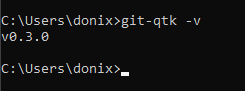
\includegraphics[width=150px]{version}
	\caption{Querying the version of the toolkit}
	\label{fig:fig-version}
\end{figure}

This will also check that a new version of the toolkit is available in the GitHub repository\cite{repo}. 

\newpage
\subsubsection{Help}
All the available commands will be displayed with description when running the program with the \textbf{-h} or \textbf{-help} flag.

\begin{figure}[H]
	\centering
	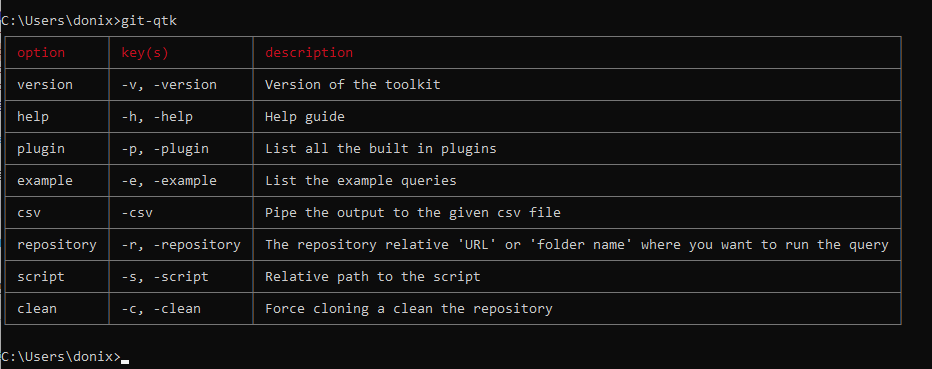
\includegraphics[width=350px]{help}
	\caption{Help of the tool}
	\label{fig:fig-help}
\end{figure}

\subsubsection{Plugin}
With the \textbf{-p} or \textbf{-plugin} flag you will be able to access all the models provided by the tool kit.

\begin{figure}[H]
	\centering
	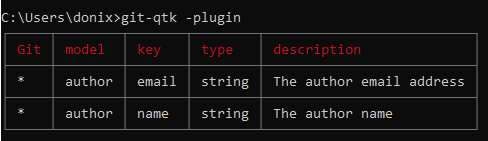
\includegraphics[width=300px]{plugin}
	\caption{List of the models provided by built in plugins}
	\label{fig:fig-plugin}
\end{figure}

\subsubsection{Examples}
To get example queries as reference, you can use the \textbf{-e} or \textbf{-example} flag.

\begin{figure}[H]
	\centering
	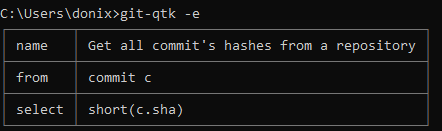
\includegraphics[width=300px]{examplee}
	\caption{An example query}
	\label{fig:fig-example}
\end{figure}

\subsubsection{Running a query}
To run a query on a specified repository you must provide the following information for the tool kit:

\begin{itemize}
	\item \textbf{-r} or -\textbf{repository} to specify which repository history should be parsed. You can give a local folder relative path or a full URL which will be cloned.
	\item \textbf{-s} or -\textbf{script} to specify which query you want to run. You can give a relative path to the query file.
\end{itemize}

This will run the query on the given repository, and the result will be printed to the standard output by default.

\begin{figure}[H]
	\centering
	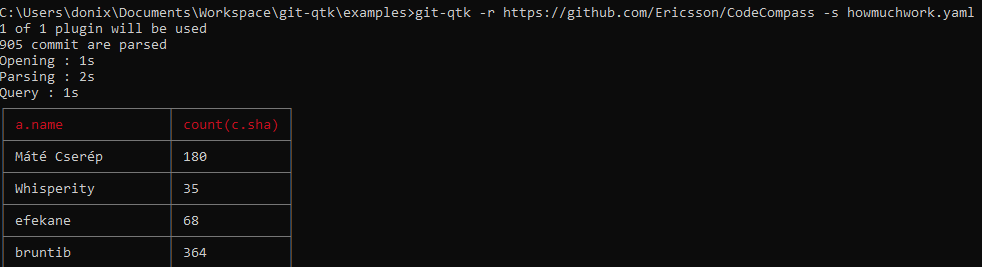
\includegraphics[width=420px]{query}
	\caption{Part of the output}
	\label{fig:fig-query}
\end{figure}


\subsection{As a Node.js library}

The toolkit is Node.js package, so it can be used as a library in any project.
Three classes are exposed by the package API which are:

\begin{itemize}
	\item Query
	\item \textit{Plugin (Abstract)}
	\item \textit{Model (Abstract)}
\end{itemize}

To use the toolkit, you have to create an instance of the \textit{Query} class by using its constructor.
The first parameter should be an \textit{Object} with all the user defined settings. 
You can use all the flags (not CLI exclusive) which are mentioned in the \textit{As a CLI tool} section.
An example would be:

\lstinputlisting[caption={lib/app.js}]{../lib/app.js}

In this way, the toolkit will clone or use the repository in the root directory of the app, this can be changed with \textbf{root} parameter.
As you can see, the parse and the query can be called separately. In this way, you are able to run multiple queries on the same parsed history.
But note, that the fist query script will determine which \textit{Plugin}s are used for the history parsing, and if you try to run a script, which
uses an unused \textit{Plugin}, it will throw an \textit{Error}. With the \textbf{useall} parameter, you can force the parser to use all \textit{Plugin}s.

\subsubsection{\label{Extending with plugins}}

\textit{Plugin}s are the parsers for which is used by the global HP (History parser). 
By default, the \textit{Git} plugin is provided to the user, but the users are able to create their own plugin as well.
\newline
This can be done by inheriting from the \textit{Plugin} class and also creating their \textit{Model}s, and passing it as a parameter for the \textit{Query}.

The plugin has a few functions, which have to be implemeted:
\begin{itemize}
	\item \textit{name()} - the name of the plugin as a string
	\item \textit{functions()} - a list of the functions which are injected into the statements
	\item \textit{reductors()} - a list of the reductors which are injected into the statements
	\item \textit{models()} - a list of the instantiated models
 
	\item \textit{init()} - run at the start of the parsing
	\item \textit{parse(db, commit)} - run for each commit
	\item \textit{post()} - run at the end of the parsing
\end{itemize}

A \textit{Model} represents a structure how the data should be stored in the database.
The model requires to implement these:
\begin{itemize}
	\item \textit{name()} - the name of the model
	\item \textit{model()} - the model definition as a name-type object 
	\item \textit{key()} - the unique key of the model
	\item \textit{parse(input)} - the processor which creates the actual database object
\end{itemize}

An example for a custom plugin:\newline
Task: We want to create a plugin, which can track the size of each commit. 
Solution:\newline

First, let's create the structure for the database object:
\lstinputlisting[caption={lib/comsize.js}]{../lib/comsize.js}

Now, we have to create the actual plugin:
\lstinputlisting[caption={lib/size.js}]{../lib/size.js}

After that we are able to pass the newly created plugin to the \textit{Query}:
\lstinputlisting[caption={lib/main.js}]{../lib/main.js}

By running the program for any repository with the following script, we will get a result which looks like this:

\lstinputlisting[caption={lib/size.yaml}]{../lib/size.yaml}


\begin{figure}[H]
	\centering
	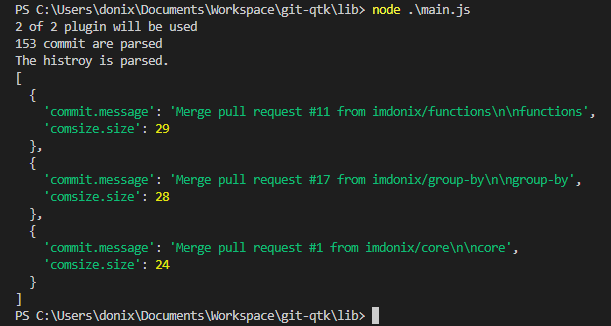
\includegraphics[width=420px]{cusplug}
	\caption{The output with the custom plugin}
	\label{fig:fig-cusplug}
\end{figure}


\section{Use cases / Examples}

In this section, you will be able to see some real world examples which use the Git plugin only.
If you want to see more, you can visit the \textbf{examples} folder.

\subsection{Use case: Who changed, what files}

We want to see who changed what file in the repository:

\begin{lstlisting}[caption={whochanged.yaml}]
	from: author a; commit c; file f
	select: a.name; f.path; short(c.date)
	where: a.email == c.author && c.changes.indexOf(f.path) >= 0
\end{lstlisting}

\subsection{Use case: A single person's commits}

We want to search for a single person's commits:

\begin{lstlisting}[caption={authorcommits.yaml}]
	from: author; commit
	select: commit.sha
	where: author.email == 'tejohnson@google.com' && commit.author == auhtor.email
\end{lstlisting}

\subsection{Use case: How many commits the authors have}

We want to see how many commits the repository authors have:

\begin{lstlisting}[caption={howmuchwork.yaml}]
	name: How much work [have] people done
	from: author a; commit c
	select: a.name; count(c.sha)
	where: a.email == c.author
	group: a.name
\end{lstlisting}